\chapter{ĐO BIẾN DẠNG SỬ DỤNG STRAIN GAGE}

\section{Mục đích thí nghiệm}
\begin{itemize}
	\item Tìm hiểu cách sử dụng strain gage để đo biến dạng.
	\item Tìm hiểu mạch đo sử dụng strain gage (mạch cầu Wheatstone).
\end{itemize}

\section{Các dụng cụ}
\begin{itemize}
	\item Thanh nhôm lắp console có các strain gage dán tại vị trí gần đầu cố định, đầu tự do của cơ cấu mang các khối nặng.
	\item Các quả nặng có đánh số, thước đo chiều dài, thước cặp.
	\item Testboard, điện trở, bộ nguồn AC, đồng hồ multimeter.
\end{itemize}

\section{Các bước tiến hành}

\begin{table}[ht]
	\centering
	\caption{Bảng kết quả đo của mạch cầu 2 strain gage}
	\begin{tabular}{lll}\toprule
		\multirow{2}{*}{STT} & \multicolumn{2}{l}{Mạch cầu 2 strain gage}\\ \cmidrule{2-3}
		& Điện áp $ V_{read}\unitp{mV} $ & Khối lượng $ M\unitp{kg} $\\\midrule
		1 & 0.51 & 0.13 \\
		2 & 0.65 & 0.28 \\
		3 & 0.97 & 0.60 \\
		4 & 1.31 & 0.95 \\
		5 & 0.99 & 0.63 \\
		6 & 0.84 & 0.48 \\
		7 & 1.93 & 1.6 \\
		8 & 2.35 & 2.03 \\
		9 & 2.22 & 1.9 \\
		10 & 0.4 & 0 \\\bottomrule
	\end{tabular}
\end{table}

\section{Đánh giá kết quả}

\begin{figure}[h]
	\centering
	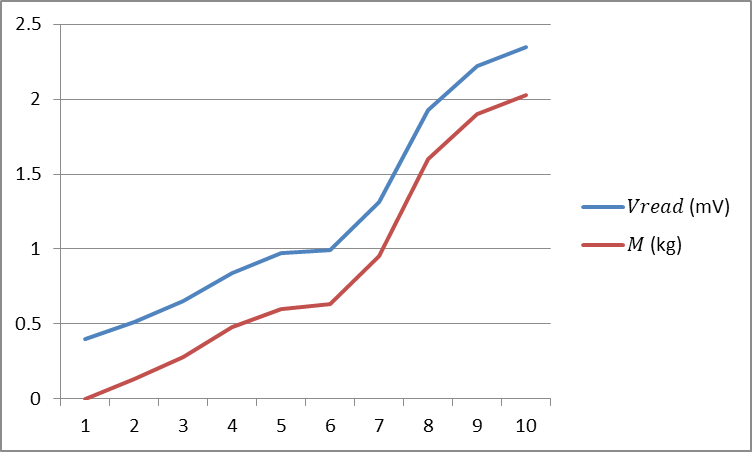
\includegraphics[width=0.75\linewidth]{images/screenshot002}
	\caption{Đồ thị mối liên hệ giữa lực và điện áp theo chiều thuận nghịch}
\end{figure}

Nhận xét biểu đồ:
\begin{itemize}
	\item Từ đồ thị ta có thể thấy mối liên hệ giữa khối lượng và điện áp là gần như tuyến tính.
	\item Kết quả xấp xỉ này xảy ra là bởi vì điện áp không ổn định.
\end{itemize}

Giải thích lý do điện áp không ổn định:
\begin{itemize}
	\item Do nhiễu trong quá trình đo.
	\item Do điện áp nhỏ nên chênh lệch điện áp cũng nhỏ.
	\item Thiết bị đo không ổn định.
	\item Sai số từ quả cân.
\end{itemize}
Biện pháp làm tăng độ ổn định: tăng độ nhạy của strain gage.

Giải thích hoạt động của mạch đo biến dạng sử dụng strain gage ở hình 10.5 trong sách hướng dẫn.
\begin{itemize}
	\item Strain gage bị ảnh hưởng bởi nhiệt độ, dán theo phương vuông góc với phương biến dạng.
	\item Đặc tính bù nhiệt của cầu: phần lớn các miếng đo biến dạng hiện nay đều có khả năng tự động cân bằng. Miếng đo được cân bằng cho phép về lý thuyết sẽ không cho thấy sự thay đổi điện trở nào khi miếng thép mà miếng đo được dán lên sẽ giãn nở khi nhiệt độ thay đổi.
	\item Đặc tính tự cân bằng này có được nhờ việc xử lý nhiệt áp dụng cho kim loại dung để chế tạo miếng đo. Cách xử lý nhiệt này chỉ có hiệu quả trong một tầm nhiệt độ giới hạn nào đó.
	\item Bằng cách dùng cầu Wheatstone ta cũng có thể chế tạo mạch cân bằng nhiệt độ. Sự thay đổi nhiệt độ của hai nhánh cầu kề nhau sẽ tự triệt tiêu nên miếng đo cân bằng được nối vào mạch cầu Wheatstone với miếng đo hữu công.
	\item Vì miếng strain gage cũng biến dạng nên ta nên dán hai miếng strain gage phía trên và phía dưới thanh để bù trừ sai số.
\end{itemize}